\begin{document}
\section*{7/4. Csőfal hőszigetelésének számítása}


\addcontentsline{toc}{section}{7/4. Csőfal hőszigetelésének számítása}

\begin{tabular}{ | p{3cm} | p{12cm} | } 
	\hline
	Zelovics Szabolcs NS9IZH  & \\  \\
	\hline
	Vegyészmérnök BSC  & \\  \\
	\hline
	Félév & 2019/2020 II. (tavaszi) félév \\ 
	\hline
\end{tabular}
\vspace{0.5cm}

\noindent Pincében falon kívül felszerelt $\SI{1/2}{\inch}$ melegvíz vezetéket samottal szigetelnek. Hogyan változik a hőveszteség a szigetelés vastagságával?$D_k_r_i_t$ = ? . Hogyan változik üvegszálas szigetelés használatakor?

\subsubsection{Adatok}
\begin{equation*}
	$d_k = \SI{0,0215}{\meter}$, $t_f_l = \SI{65}{\celsius}$
	\quad 
	 $\alpha_1 = \SI{11,6}{\watt\per\meter\cubed\kelvin}$, 
	\quad
	$t_l_e_v = \SI{5}{\celsius}$,
	\quad
	$\lambda_s = \SI{0,47}{\watt\per\meter\kelvin},
	\quad
	$l_u = {0,07}{\inch}$
\end{equation*}

\noindent Gyakorlatban a csőfal termikus ellenállása a szigetelés mellet elhanyagoltható, ennek figyelembevételével a lineáris hőáram:
\begin{equation*}
	 \dot{q_l} = \frac{T_1 - T_2}{\frac{ln(\frac{D}{dk})}{2\pi\lambda}+\frac{1}{\alpha D\pi}}
\end{equation}

\noindent A kritikus átmérő 
\begin{equation*}
D_k_r_i_t = \frac{2\lambda}{\alpha}
\end{equation*}

$D_K_s_a_m = \SI{0,081034}{\meter}$

$D_K_u_v = \SI{0,00687}{\meter}$



\begin{tabular}{ | p{2cm} | p{2cm} | p{3cm} | p{3cm} | } 
	\hline
	D & \szigma & q(W/m) & q(W/m) \\
	\hline
	mm & mm & samott & üvegszál \\ 
	\hline
	21,5 & 0 & 47,0164 & 47,0128 \\
	\hline
	41 & 19,5 & 67,5943 & 18,5275 \\
	\hline
	61 & 39,5 & 74,7213 & 13,0449 \\
	\hline
	81 & 59,5 & 76,1487 & 10,6827 \\
	\hline
	101 & 79,5 & 75,4187 & 9,3342 \\
	\hline
	121 & 99,5 & 73,9071 & 8,4485 \\
	\hline
	221 & 199,5 & 65,7028 & 6,3854 \\
	\hline
	321 & 299,5 & 59,9463 & 5,5336 \\
	\hline
	421 & 399,5 & 55,9479 & 5,0413 \\
	\hline
\end{tabular}


\begin{figure}[h]
	\centering
	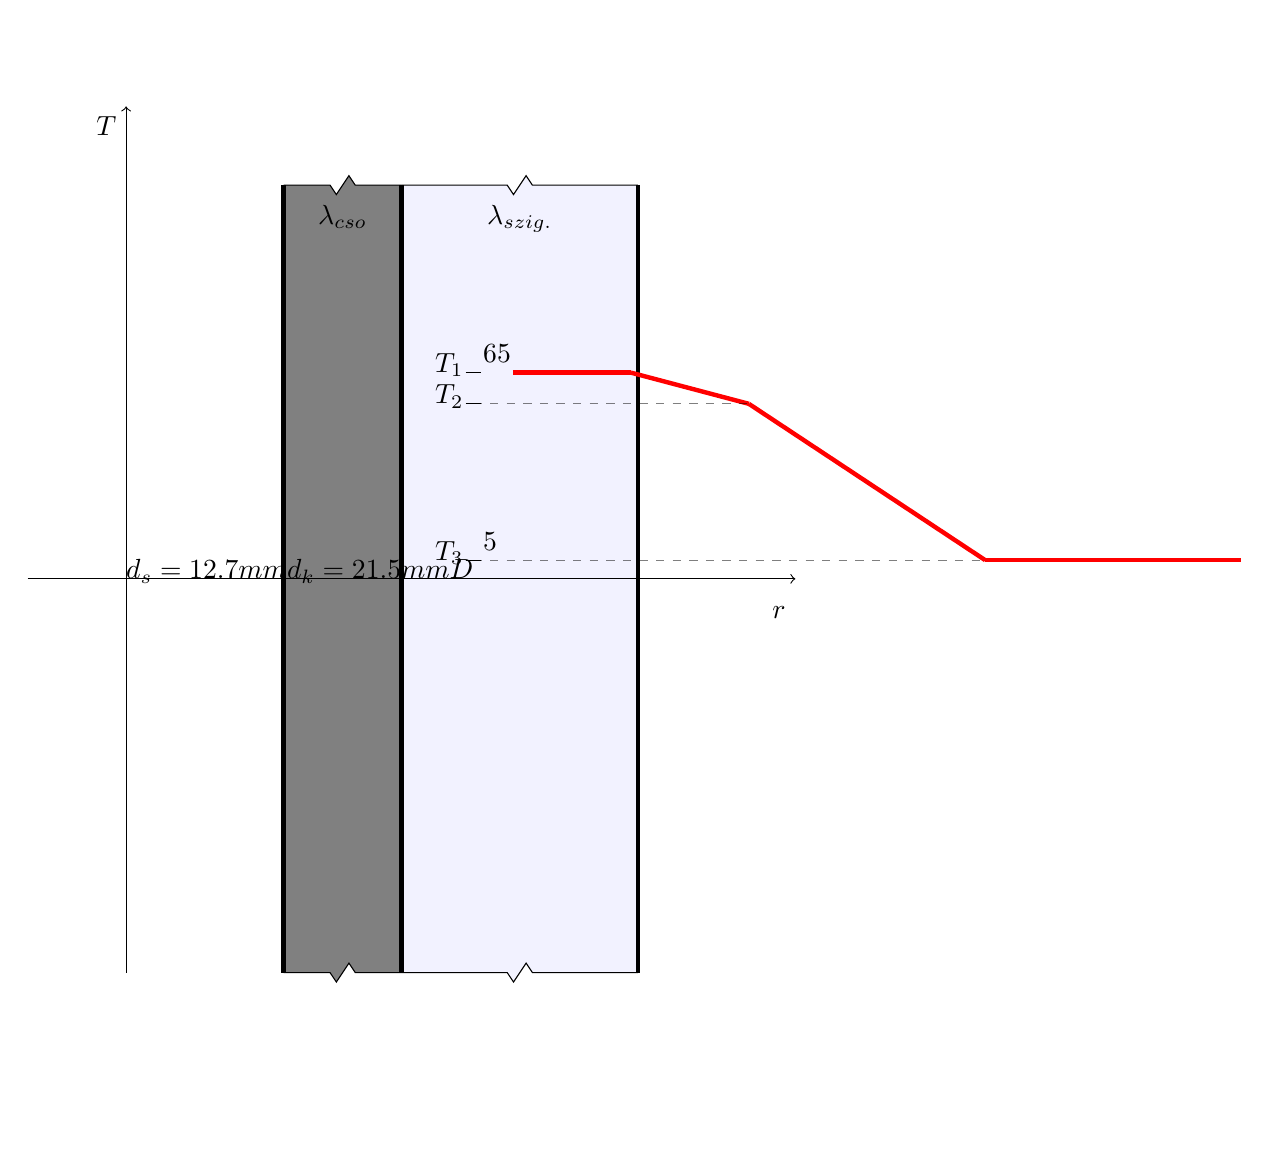
\begin{tikzpicture}
		% Fiktív értékek a vázlathoz
		\pgfmathsetmacro{\DB}{4}
		\pgfmathsetmacro{\DK}{7}
		\pgfmathsetmacro{\DJ}{13}
		\pgfmathsetmacro{\lambdaA}{8}
		\pgfmathsetmacro{\lambdaJ}{2.9}
		\pgfmathsetmacro{\alfaL}{11.5}
		\pgfmathsetmacro{\qlin}{326.815}
		
		\pgfmathsetmacro{\RA}{\DB/2}
		\pgfmathsetmacro{\RB}{\DK/2}
		\pgfmathsetmacro{\RC}{\DJ/2}
		
		\pgfmathsetmacro{\L}{5}
		
		\pgfmathsetmacro{\kelvin}{4.2}
		\pgfmathsetmacro{\TA}{11/\kelvin}
		\pgfmathsetmacro{\TB}{9.33/\kelvin}
		\pgfmathsetmacro{\TC}{1/\kelvin}
		
		% KÖRBEVÁGÁS
		\clip ({-1.25}, {-(\L)-2}) rectangle ({2.2*\RC}, {\L+2});
		
		% A csőfal és a jégréteg
		\fill[gray, opacity=100] (\RA,\L) -- ({(\RA+\RB)/2-0.16},\L) -- ({(\RA+\RB)/2-0.08}, {\L-0.12}) -- ({(\RA+\RB)/2+0.08}, {\L+0.12}) -- ({(\RA+\RB)/2+0.16}, \L) -- (\RB, \L) -- (\RB, -\L) -- ({(\RA+\RB)/2+0.16}, -\L) -- ({(\RA+\RB)/2+0.08}, {-\L+0.12}) -- ({(\RA+\RB)/2-0.08}, {-\L-0.12}) -- ({(\RA+\RB)/2-0.16},-\L) -- (\RA,-\L);
		\draw[] (\RA,\L) -- ({(\RA+\RB)/2-0.16},\L) -- ({(\RA+\RB)/2-0.08}, {\L-0.12}) -- ({(\RA+\RB)/2+0.08}, {\L+0.12}) -- ({(\RA+\RB)/2+0.16}, \L) -- (\RB, \L);
		\draw[] (\RA,-\L) -- ({(\RA+\RB)/2-0.16},-\L) -- ({(\RA+\RB)/2-0.08}, {-\L-0.12}) -- ({(\RA+\RB)/2+0.08}, {-\L+0.12}) -- ({(\RA+\RB)/2+0.16}, -\L) -- (\RB, -\L);
		
		\fill[blue, opacity=0.05] (\RB,\L) -- ({(\RB+\RC)/2-0.16},\L) -- ({(\RB+\RC)/2-0.08}, {\L-0.12}) -- ({(\RB+\RC)/2+0.08}, {\L+0.12}) -- ({(\RB+\RC)/2+0.16}, \L) -- (\RC, \L) -- (\RC, -\L) -- ({(\RB+\RC)/2+0.16}, -\L) -- ({(\RB+\RC)/2+0.08}, {-\L+0.12}) -- ({(\RB+\RC)/2-0.08}, {-\L-0.12}) -- ({(\RB+\RC)/2-0.16},-\L) -- (\RB,-\L);
		\draw[] (\RB,\L) -- ({(\RB+\RC)/2-0.16},\L) -- ({(\RB+\RC)/2-0.08}, {\L-0.12}) -- ({(\RB+\RC)/2+0.08}, {\L+0.12}) -- ({(\RB+\RC)/2+0.16}, \L) -- (\RC, \L);
		\draw[] (\RB,-\L) -- ({(\RB+\RC)/2-0.16},-\L) -- ({(\RB+\RC)/2-0.08}, {-\L-0.12}) -- ({(\RB+\RC)/2+0.08}, {-\L+0.12}) -- ({(\RB+\RC)/2+0.16}, -\L) -- (\RC, -\L);
		
		\draw[ultra thick] (\RA,-\L) -- (\RA,\L);
		\draw[ultra thick] (\RB,-\L) -- (\RB,\L);
		\draw[ultra thick] (\RC,-\L) -- (\RC,\L);
		
		% Tengelyek
		\draw[->] (0,-\L) -- (0,\L+1) node[anchor=north east]{$T$};
		\draw[->] (-1.25, 0) -- (\RC+2, 0) node[anchor=base east, shift={(0,-0.5)}]{$r$};
		
		% A hővezetési és hőátadási tényezők
		\node[anchor=base] at ({(\RA+\RB)/2},{\L-0.5}) {$\lambda_{cso}$};
		\node[anchor=base] at ({(\RB+\RC)/2},{\L-0.5}) {$\lambda_{szig.}$};
		
		% Az átmérők
		\pgflength[xa={-\RA}, ya={-\L}, xb={\RA}, yb={-\L}, alim=0, blim=1, ra=0.6]{$\diameter d_s = 12.7mm$};
		\pgflength[xa={-\RB}, ya={-\L}, xb={\RB}, yb={-\L}, alim=0, blim=1, ra=1.2]{$\diameter d_k = 21.5mm$};
		\pgflength[xa={-\RC}, ya={-\L}, xb={\RC}, yb={-\L}, alim=0, blim=1, ra=1.8]{$\diameter D$};
		
		% T(r) körülbelüli hőmérséklet-hely függvény
		\draw[red, ultra thick] (0.5,\TA) -- (\RA,\TA);
		\draw[ultra thick, color=red, domain=\RA:\RB, smooth, variable=\r] plot (\r, {\TA - ((\r-\RA)*10/9)/\kelvin});
		\draw[ultra thick, color=red, domain=\RB:\RC, smooth, variable=\r] plot (\r, {\TB - ((\r-\RB)*50/18)/\kelvin});
		
		\draw[red, ultra thick] (\RC,\TC) -- (1.5*\RC,\TC);
		
		% A hőmérséklet értékek
		\draw (-0.1,\TA) -- (0.1,\TA);
		\node[anchor=base east] at (0,\TA) {$T_1$};
		\node[anchor=south west] at (0,\TA) {$\SI{65}{\celsius}$};
		
		\draw (-0.1,\TB) -- (0.1,\TB);
		\draw[black, opacity=0.5, dashed] (0,\TB) -- (\RB,\TB);
		\node[anchor=base east] at (0,\TB) {$T_2$};
		
		\draw (-0.1,\TC) -- (0.1,\TC);
		\draw[black, opacity=0.5, dashed] (0,\TC) -- (\RC,\TC);
		\node[anchor=base east] at (0,\TC) {$T_3$};
		\node[anchor=south west] at (0,\TC) {$\SI{5}{\celsius}$};
		
	\end{tikzpicture}
	\caption*{A hőmérséklet-hely függvény vázlata.}
\end{figure}



\pagebreak
